\documentclass{scrreprt}
\usepackage{scrhack}
\usepackage[utf8]{inputenc}
\usepackage[scaled]{beramono}
\usepackage[T1]{fontenc}
\usepackage[final]{microtype}
\usepackage{hyperref}

\usepackage{color}
\definecolor{bluekeywords}{rgb}{0.13,0.13,1}
\definecolor{greencomments}{rgb}{0,0.5,0}
\definecolor{redstrings}{rgb}{0.9,0,0}

\setlength{\parindent}{0em}
\setlength{\parskip}{1em}

\usepackage{listings}
\lstset{
numbers=left,
frame=lines,
showspaces=false,
showtabs=false,
breaklines=true,
postbreak=\mbox{\textcolor{black}{$\hookrightarrow$}\space},
showstringspaces=false,
commentstyle=\color{greencomments},
keywordstyle=\color{bluekeywords}\bfseries,
stringstyle=\color{redstrings},
basicstyle=\ttfamily
}

\usepackage{graphicx}

\usepackage[
backend=biber,
style=authoryear,
sorting=ynt
]{biblatex}
\addbibresource{mendeley.bib}

\title{Programming Mobile Devices: Assignment 1}
\author{Gary Moore}

\begin{document}
\maketitle
\tableofcontents

\chapter{Inception}\label{research}

JD Electronics are requesting the development of a mobile app that promotes their company by providing features that attract the customer to download the app, with hooks to maintain their interaction with their app, and their brand.

The app is to be feature rich, which entertainment such as quiz's and other  interactive elements to keep the user engaged, along with some e-commerce features allowing the user to find information about the products that they offer, along with an interface to purchase products on there too.

\section{Challenges \& Solutions}

We will have to make a few judgments with regards to the approach taken in developing this app. With the many variables involved in mobile application development, every path we take will have advantages and disadvantages. We have to look at each option in the context of the project proposal, and what would be a best fit for the type of app we are setting out to create.

The following challenges have been identified and will be discussed below:

\begin{itemize}
    \item Platform market share
    \item Platform market potential
    \item Platform fragmentation
    \item Ease of development
    \item First and third party support of platform
    \item Software tooling
    \item Scalability
    \item Cost
\end{itemize}

The story behind the market share of each major mobile phone platform isn't simple, with the raw numbers not giving much away, with a cursory glance at the information giving the impression that the android platform may be the way to go because of it's much larger user base.

The android platform is host to the largest global market share when compared to any other mobile platform in use today. They have a market share that has consistently risen over time to in excess of 80\%, whereas the iOS market-share has remained consistent over time, hovering roughly between 10 and 20\% over the years, with a market share of 12.1\% as of Q2 2017. \cite{2017MobileStatista}.

These statistics give the impression of a very lucrative marketplace on the android platform, however this could be misleading, as research shows there's greater potential on the iOS market, as users are more likely to pay for goods on the apple app store. Going into the future, iOS looks to hold on to the title of the greatest app store revenue generator over Google Play up until 2021 \cite{2017App2021}, so in the short ot medium term, this looks like the best choice when publishing a for profit app.

Another important factor to look at is the friction of trade. Both iOS and Android have a mobile payment system that is used to make online and in store payments easier, and more intuitive. Less friction during a trade, that is the hoops the user is required to go through before making a purchase, is significantly reduced when using these systems which has the effect of increasing the conversion rate on e-commerce focused websites and apps.

The iOS platform has the biggest market-share between Android/Google Pay and Apple Pay, \cite{2017UserStatistic}, this means that iOS users will be more likely to follow through with a purchase, as payment simply involves holding their thumb over a fingerprint reader.

iOS should be the initial development target, however work on developing an android further should be looked into in the future, as there still is a significant market that could be utilized there.

\section{Opportunities \& Challenges}

The mobile app development world is a chance to penetrate a new marketplace, with new marketing and commerce opportunities available to a different audience compared to traditional brick and mortar, and the website. On iOS, there is the opportunity to be featured on the main page, which is great for exposure and growth, however this likely won't happen unless the app is really excellent. Android provides similar functionality, however the featured app editorials are less obvious on the store, and users are less likely to click them.

There's the opportunity with a mobile app to get access to features that would not work on a website. For example, TouchID login on an iPhone, and push notifications on both platforms allow a reach to the customer that gives you the opportunity to increase your conversion rate at the cart by gently reminding the user that they abandoned their cart, and enabling friction-less payments with apple and Google pay with biometric login.

Another useful feature that push notifications facilitates is shipping updates from a shipping information REST API, keeping the user informed as to what is happening with their package, which makes it more likely that the user will come back to shop again after having a positive experience.



\section{Platforms \& Devices}

Coming out of the abstract and into the development of the app, there are many tools for the job. The big examples of these are the following:

\begin{itemize}
    \item Microsoft Xamarin Studio
    \item Apache Cordova
    \item React Native
\end{itemize}

\paragraph{Xamarin Studio}

Xamarin is a great platform for those that are native to the windows platform and .NET framework. Those familiar with C$^\sharp$ get to work with the language they are familiar with, without the factor of looking up documentation slowing down the development process. There are plenty of people with a skill set in .NET, with transferable skills to a mobile development project, such as experience with the MVC\footnote{Model View Controller} mode of development. Xamarin offers full integration of apple and Google native APIs into the .NET framework, along with UI elements, which means that there is no concern with this development platform with divergence from native APIs and the problems that causes, such as feature, performance and visual differences.

A great time saving feature of visual studio is the nuget package manager integrated into Visual Studio Community for Windows, and for macOS. This is a package manager much like APT in Ubuntu or Debian that allows you to download, manage and update frameworks and libraries that your project uses. It could be argued that you could just use \texttt{git submodule add --init --recursive}, however a package manager integrated into the IDE is easier to use, and doesn't create as much confusion for new developers on the platform.

There is one issue with Xamarin that could hold the project back in the future, and that is the requirement for diverging code bases when it comes to the interface development if you want to use native interface elements in optimal positions on each app. Xamarin Forms works the create the UI for both with one code base, but it can be slow on bigger projects, and could prohibitively slow down development and maintenance of the app in the future.

There is also another great version of Xamarin Studio on macOS, which offers much the same functionality as Visual Studio on windows for multiplatform app development.

\paragraph{Apache Cordova}

This development technology allows the developers to create mobile apps using web APIs such as javascript, HTML, and CSS to develop their application. This creates what is considered a hybrid app, which acts much like a web page, however it is run locally on the device, with access to the platform specific APIs that allow you to do more than a website ever could, such as send push notifications, or gather information from the mobile phones various sensors.

One of the advantages of using this approach is the ability to use a lot of the great JavaScript libraries made for the web in your application, enriched with the new telemetric data available from the phone.

JavaScript is an interpreted langauge, which is a disadvange as the phone translates each plain text statement one line at a time rather than taking a pre-compiled down to machine code approach of Swift or JVM languages like Java and Kotlin\footnote{The new language introduced into Android Studio}.

This could be a great option for any company that already has a website in use, as there is a great degree of data portability that this supports. Any client-side code and HTML/CSS on the website of a company made for mobile can be used on the mobile app, saving money and time in the upfront cost of getting a mobile app up and going.

\paragraph{React Native}

Web developers using the most modern technologies with be familiar with react, which is a framework that extends javascript. The advantage of developing with this framework, is the removal of the need to recompile the application over and over again in the write $\rightarrow$ compile $\rightarrow$ debug loop. Again, this has the same issues as cordova, with slower code execution time, which is only really an issue with complicated math functions, of performance constrained code, such as animation.

For apps that interact with the web a lot, this is less of an issue, as HTTP GET requests etc. are typically performed asynchronously from the main thread which handles animation etc, with the tasks being done when their done without slowing down the rest of the app.

\paragraph{Xcode}

Xcode is the easiest set of tools to work with for mobile application development, with swift being a smart language that offers modern features such as closures (comparable to lambda expressions in other languages), type safety with type inference, generics, and other nice syntactic sugar like string interpolation. Swift is also a fast language (not fast to compile), which is run on cutting edge mobile processor technology with the latest frameworks almost always available to you, due to the lack of OS fragmentation on the iOS platform.

The development model of a view, view controller and model just makes a lot of sense too, providing a good framework to discreetly abstract different types of logic that increase code readability.

This is in a lot of ways the mobile developers platform, with a lot of sophistication in hardware, and great apple APIs and programming language. It does however come with it's drawbacks. Swift is open source and on different platforms, however it's only likely to take off on apples platform, whereas .NET is quickly opening up to be a dominant framework on multiple platforms. You need a mac to develop with Xcode for iOS. The apple app store can be a little restrictive on the app store when it comes to software that allows runtime code execution. Objective-C still has better auto-completion support in Xcode when compared to the newer sibling, however this is more than made up for with the removal of the remarkable amount of square brackets and the little amount of memory management required with the language.

\paragraph{Android Studio}

This is a relatively new IDE from Google based on JetBrains ReSharper IDE for Java. This IDE supports a lot of advanced features comparable to the features in Xcode, and can also do more than the iOS cousin, with language support for Java and Kotlin, however the issue with Android Studio and android development in general is the enormous OS fragmentation on the platform, with the latest features often not being able to be used in order to maintain compatibility with older platforms. Android development is a mess, with the Gradle build system downloading gigabytes of dependencies anytime you change your API target.

Developing for android might be useful if you have a good marketing budget and don't expect to make money through the app, only raise awareness or offer a service driving people towards your platform.

\section{Addressing User Requirements}

The user is looking an application to promote their business, with the specific requirements of what the application is to do being a little vague. We are proposing an e-commerce application for the company, which has a login and registration system, product listings, a product detail view for every product, and the ability to add to and manage a cart before purchase.

A mock-up will be built on the app inventor platform, demonstrating the features that the application will be capable of. This tool allows for the quick prototyping of applications through the use of drag and drop elements that exist at a high level of abstraction, removing much of the work on the details often required when working in software such as Xcode or Android Studio.

\section{Scalability \& Feasibility}
% how scalability will be considered for potential future development and discussion of the different aspects of Competitive Advantage, Integration, feasibility and cost and add value mobile technologies like location awareness, camera, scanning etc.

It would be ideal for the product to be built on top of a cloud scaling system like Kubernetes\footnote{https://kubernetes.io/}, which allows the instantiation and termination of virtual machines based on the demand of the application. You can use a platfrom like Google Cloud Platform\footnote{https://www.google.com/} to manage all these variables for you.

There's now the concept of the backend in the cloud for mobile devices that provide services like authentication for login, social networking, database integration and several other great APIs that can scale with the size of your business.

Integration with the cloud will have to happen with any application integrated into the internet at some point, so it's good the get this done at the development stage before it becomes too much of a hassle to do.

\section{Cost}

The cost of development is going to vary from platform to platform, with the most expensive form of development probably being 2 independant teams for android and iOS development, and the most cost effective solution being adopting the web technologies currently used by the company into an app created with the cordova framework from apache. Both are valid options, with their advantages and disadvantages, however I feel that the best approach for a multiplatform app, is to use a framework that is suited for multiplatform development on mobile apps.

The most developed out of these frameworks is likely the .NET framework with xamarin. There are plenty of .NET developers out there in the world, and with the open sourcing of the .NET framework and the creation of the .NET Foundation, the framework has seen great support on other platforms such as macOS since then, with a version of Xamarin studio available on Windows, macOS and different distributions of GNU/Linux for a few years now. You could cut the size of the required staff significantly, with only one code base being required.
\chapter{Design}\label{design}

\section{Pseudocode}

\subsection*{Welcome Screen}

\begin{lstlisting}
When login button tapped:
    Go to the login screen
    
When register button tapped:
    Go to register screen
\end{lstlisting}

\subsection*{Register Screen}

\begin{lstlisting}
When system back button pressed:
    Go to welcome screen
    
When application back button pressed:
    Go to welcome screen

When submit button pressed:
    If the password input matches the confirmation input:
        Set the hidden error label to visible
        Store the username from textbox into TinyDB with the tag ('username' prefix + actual username)
        Store password from textbox into TinyDB with the tag ('password' prefix + actual password)
        Set success label visibility to true
        Set password error label visibility to false
\end{lstlisting}

\subsection*{Login Screen}

\begin{lstlisting}
When system back button is pressed:
    Go back to welcome screen
    
When application back button is pressed:
    Go back to welcome screen
    
When login button is pressed:
    I username and password match a username and password retrieved from the database:
        open the main product view screen
    else:
        set error label visibility to true
\end{lstlisting}

\subsection*{Main Screen}

\begin{lstlisting}
Initialize global variable 'products' to JSON format collection of products and their details in key: string pairs

When cart button is pressed:
    Open the cart screen
    
When system back button is pressed:
    Open the welcome screen
    
After picking item in product list:
    Store global 'products' in TinyDB with tag 'Products'
    Store the users selection in TinyDB with tag 'ProductValue'
    Open the Product View screen

When the Main screen is loaded:
    Call getTitlesFromList function
    Set the list view of products elements to the list returned from getTitlesFromList

function getTitlesFromList:
    initialize local 'listOfTitles' to empty list
    for each 'number' in list 'products':
        Get the list at 'number' in 'products'
        In this new list, select the item at it's first index
        add this item to the list 'listOfTitles'
    return 'listOfTitles'
\end{lstlisting}

\subsection*{Product View Screen}

\begin{lstlisting}
initialize global 'products' to TinyDB item at tag 'Products'
initialize global 'selection' to TinyDB item at tag 'ProductValue'
initialize global 'product' to result of getProductList using key global 'selection' and list global 'products'

When system back button is pressed:
    Go to main screen page
    
When add to cart button pressed:
    Initialize local 'workingList' to empty list
    Set 'workingList' to TinyDB entry at tag "Cart"
    Add global 'selection' to list 'workingList'
    Store the working list to TinyDB under the tag 'Cart'
    Call on snackbar extension to print 'Added to Cart' when add to cart button is pressed

On screen initialize:
    Set product title label text to global 'selection' with html h1 formatting
    set product description label text to the item at key 'Description' in list global 'product' with html h2 formatting
    Set product price label text to the item at key 'Price' in the list global 'product'
    if selection == "Piping Simulator 2018":
        set product image to "pipingSimulator2018.png"
    else if selection == "Sprug Nuts":
        set product image to "sprugNuts.jpg"
    else if selection == "Electronic Game":
        set product image to "electronicGame.jpg"
    else if selection == "Donald Trump: The Board Game":
        set product image to "trumpGame.jpg"
        
function getProductList takes 'key', 'list':
    Initialize local variable called 'workingList'
    Set 'workingList' by getting value using look up in pairs block using 'key' and 'list'
    return 'list'
\end{lstlisting}

\subsection*{Cart Screen}

\begin{lstlisting}
Initialize global 'products' to empty list
Initialize global 'cart' to empty list

When system back button pressed:
    Open screen main
    
When home button pressed:
    Open screen main
    
When clear button pressed:
    Clear cart database
    Clear cart listView
    
On screen initialize:
    Set 'products' to value from database
    Set 'cart' to value from database
    Call function populateCart
    
Function populateCart:
    Initialize local 'cartListView'
    For each 'item' in 'cart':
        Select item from 'cart' based on 'item' as index
        Use above item as key for item from pair in list 'products'
        Find value in pair with key "Price"
        The cart item and price item will be concatenated in string and added to list
    Set 'cartListView' as elements for the cart list
\end{lstlisting}

\section{Flow Charts}

\subsection*{Registration}

\begin{center}
    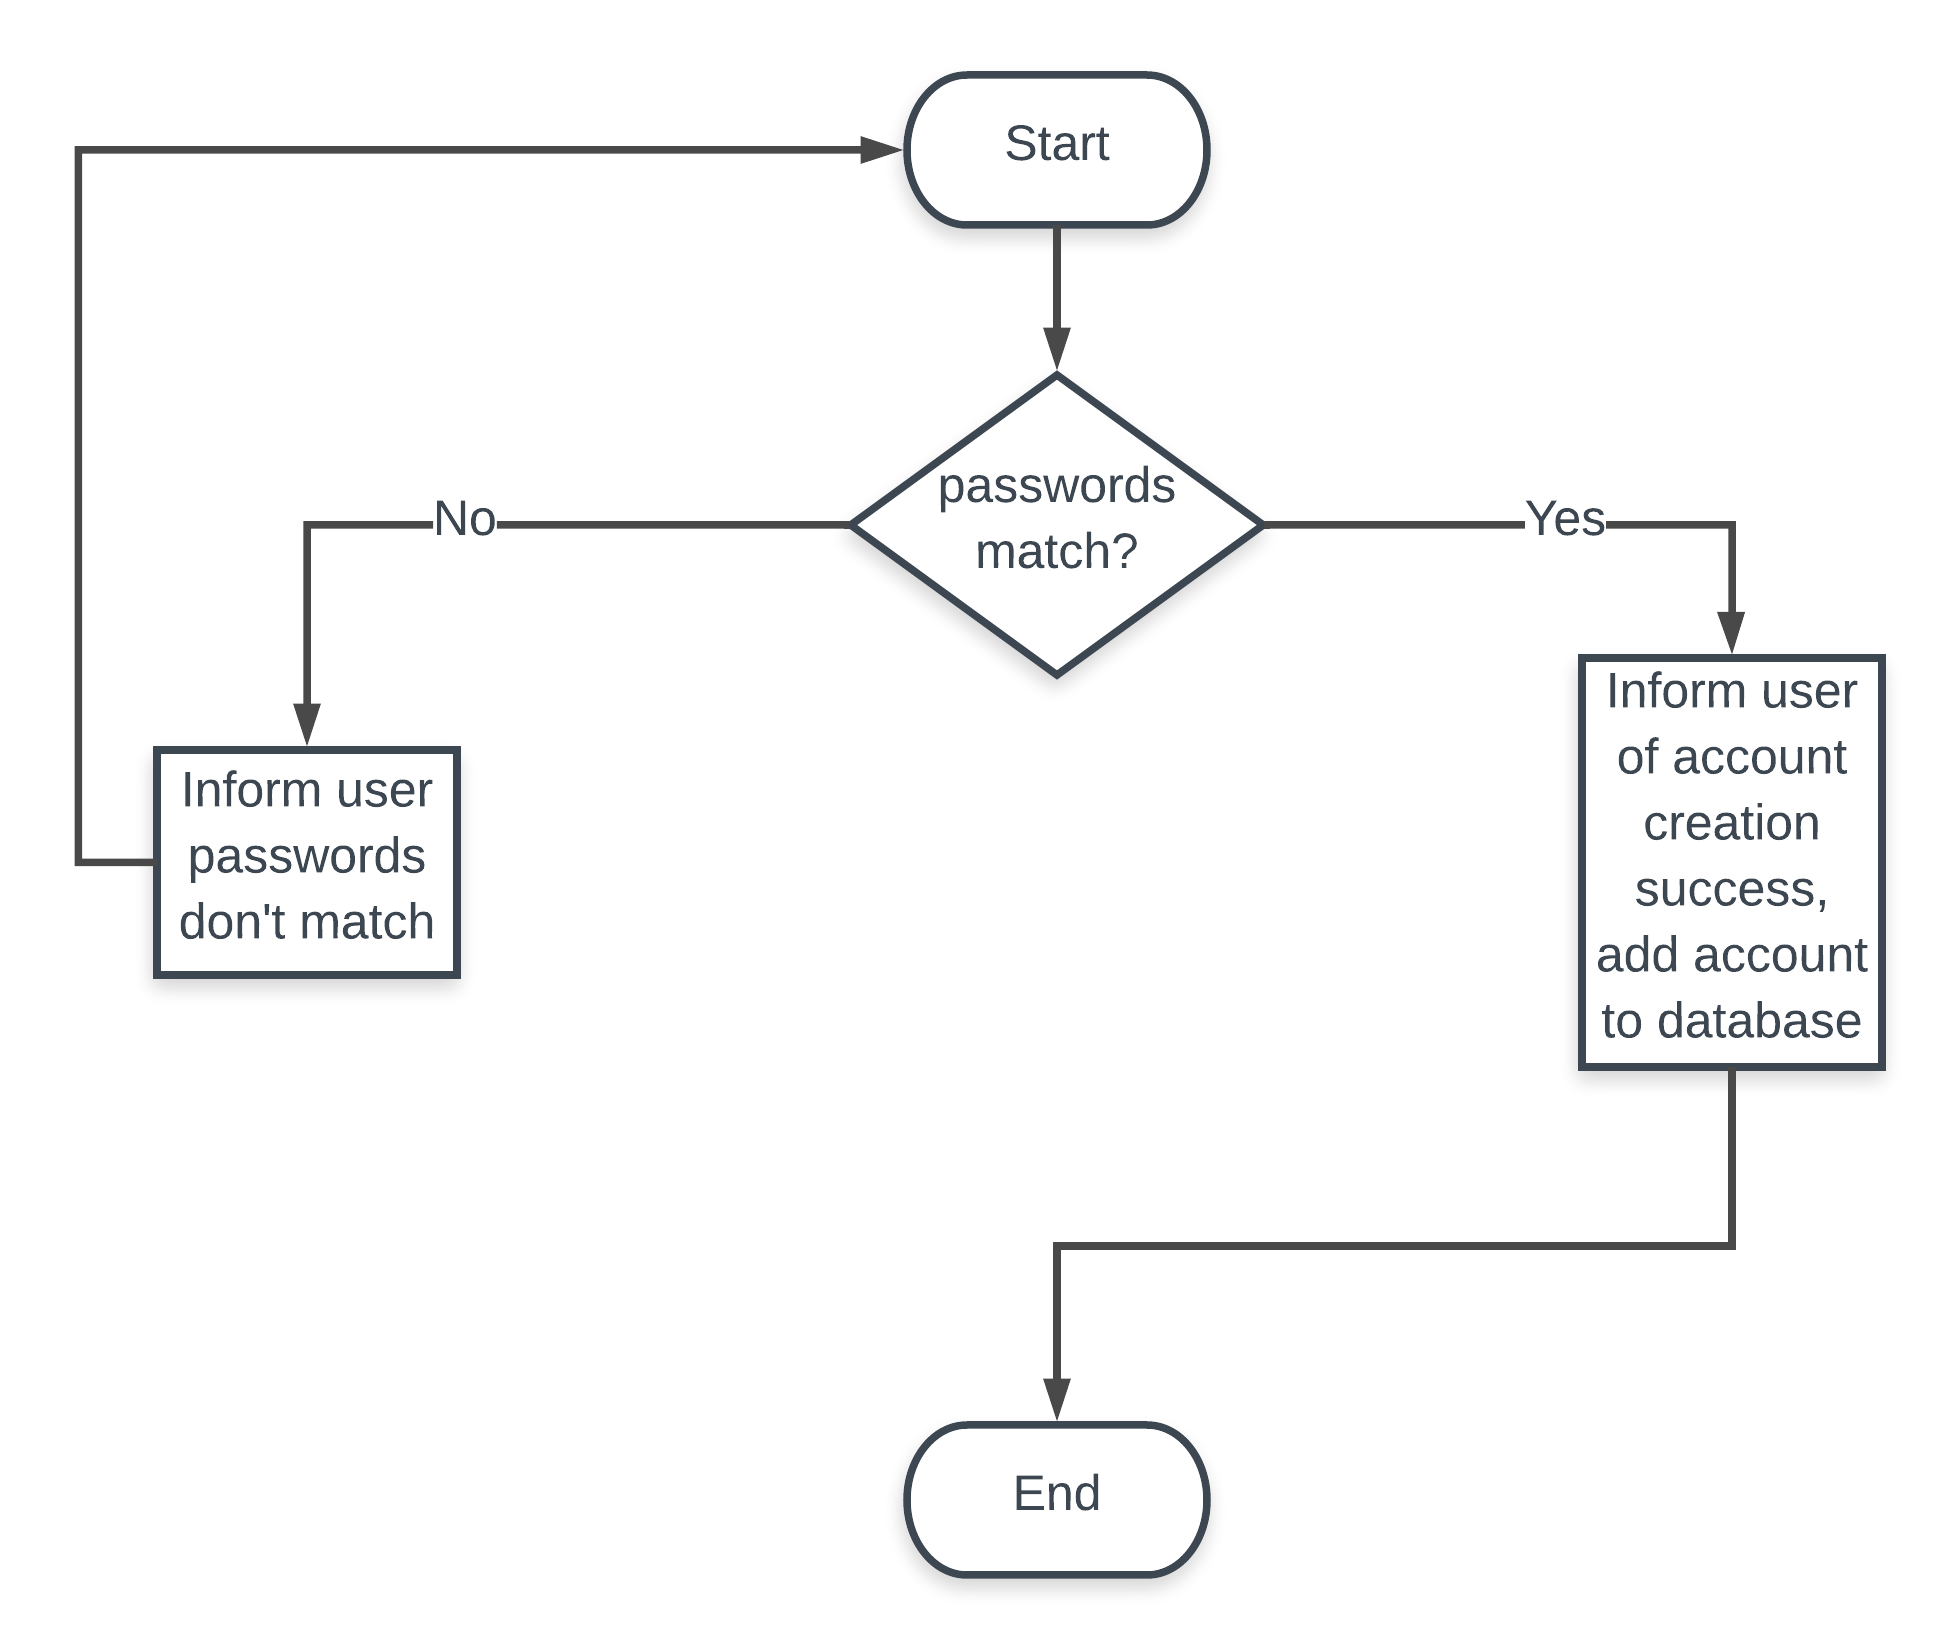
\includegraphics[width=0.9\linewidth]{images/flowRegister.png}
\end{center}

\subsection*{Login}

\begin{center}
    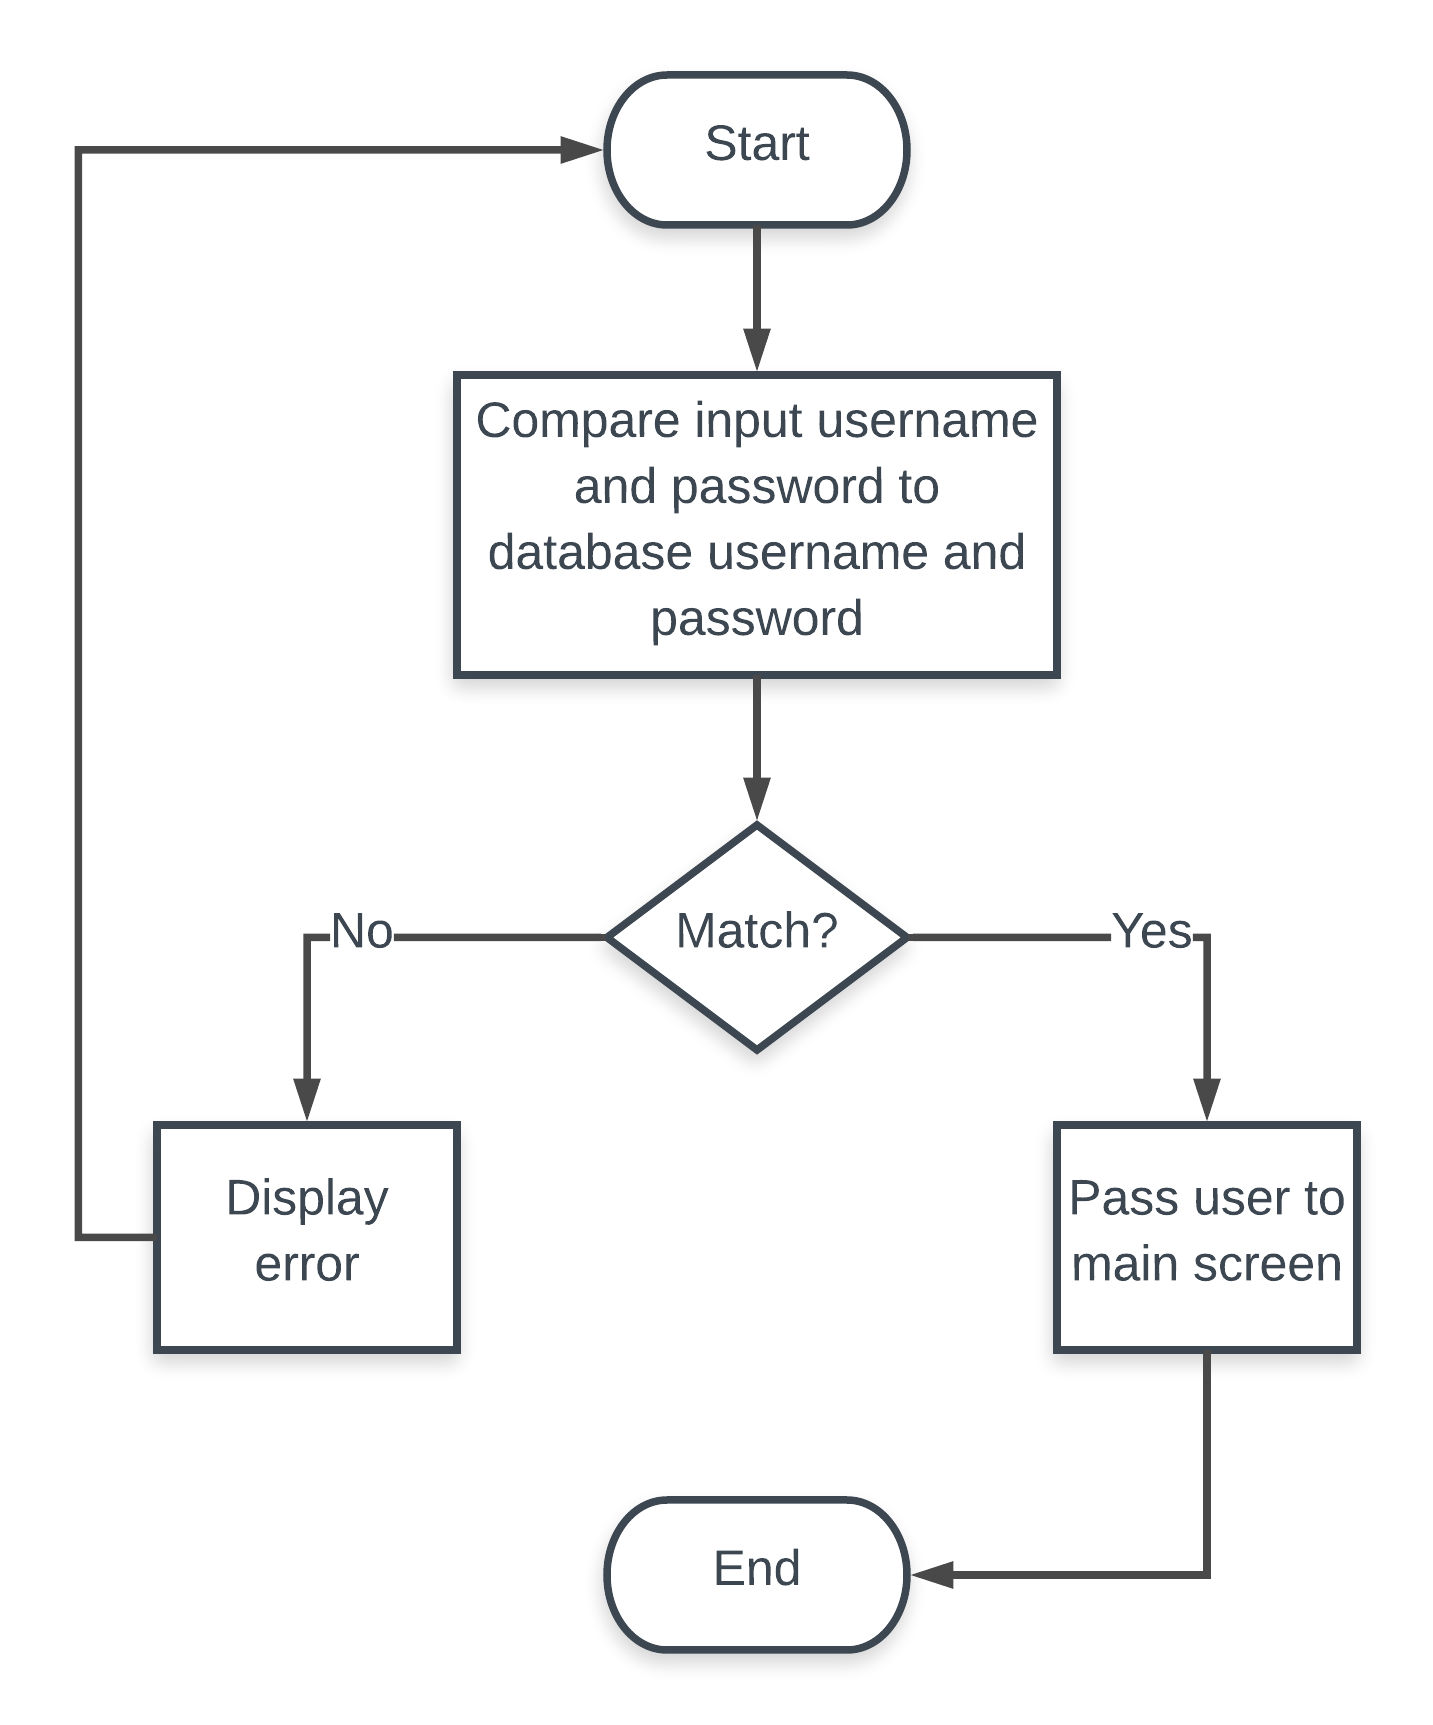
\includegraphics[width=0.9\linewidth]{images/flowLogin.png}
\end{center}

\subsection*{Main Page}

\begin{center}
    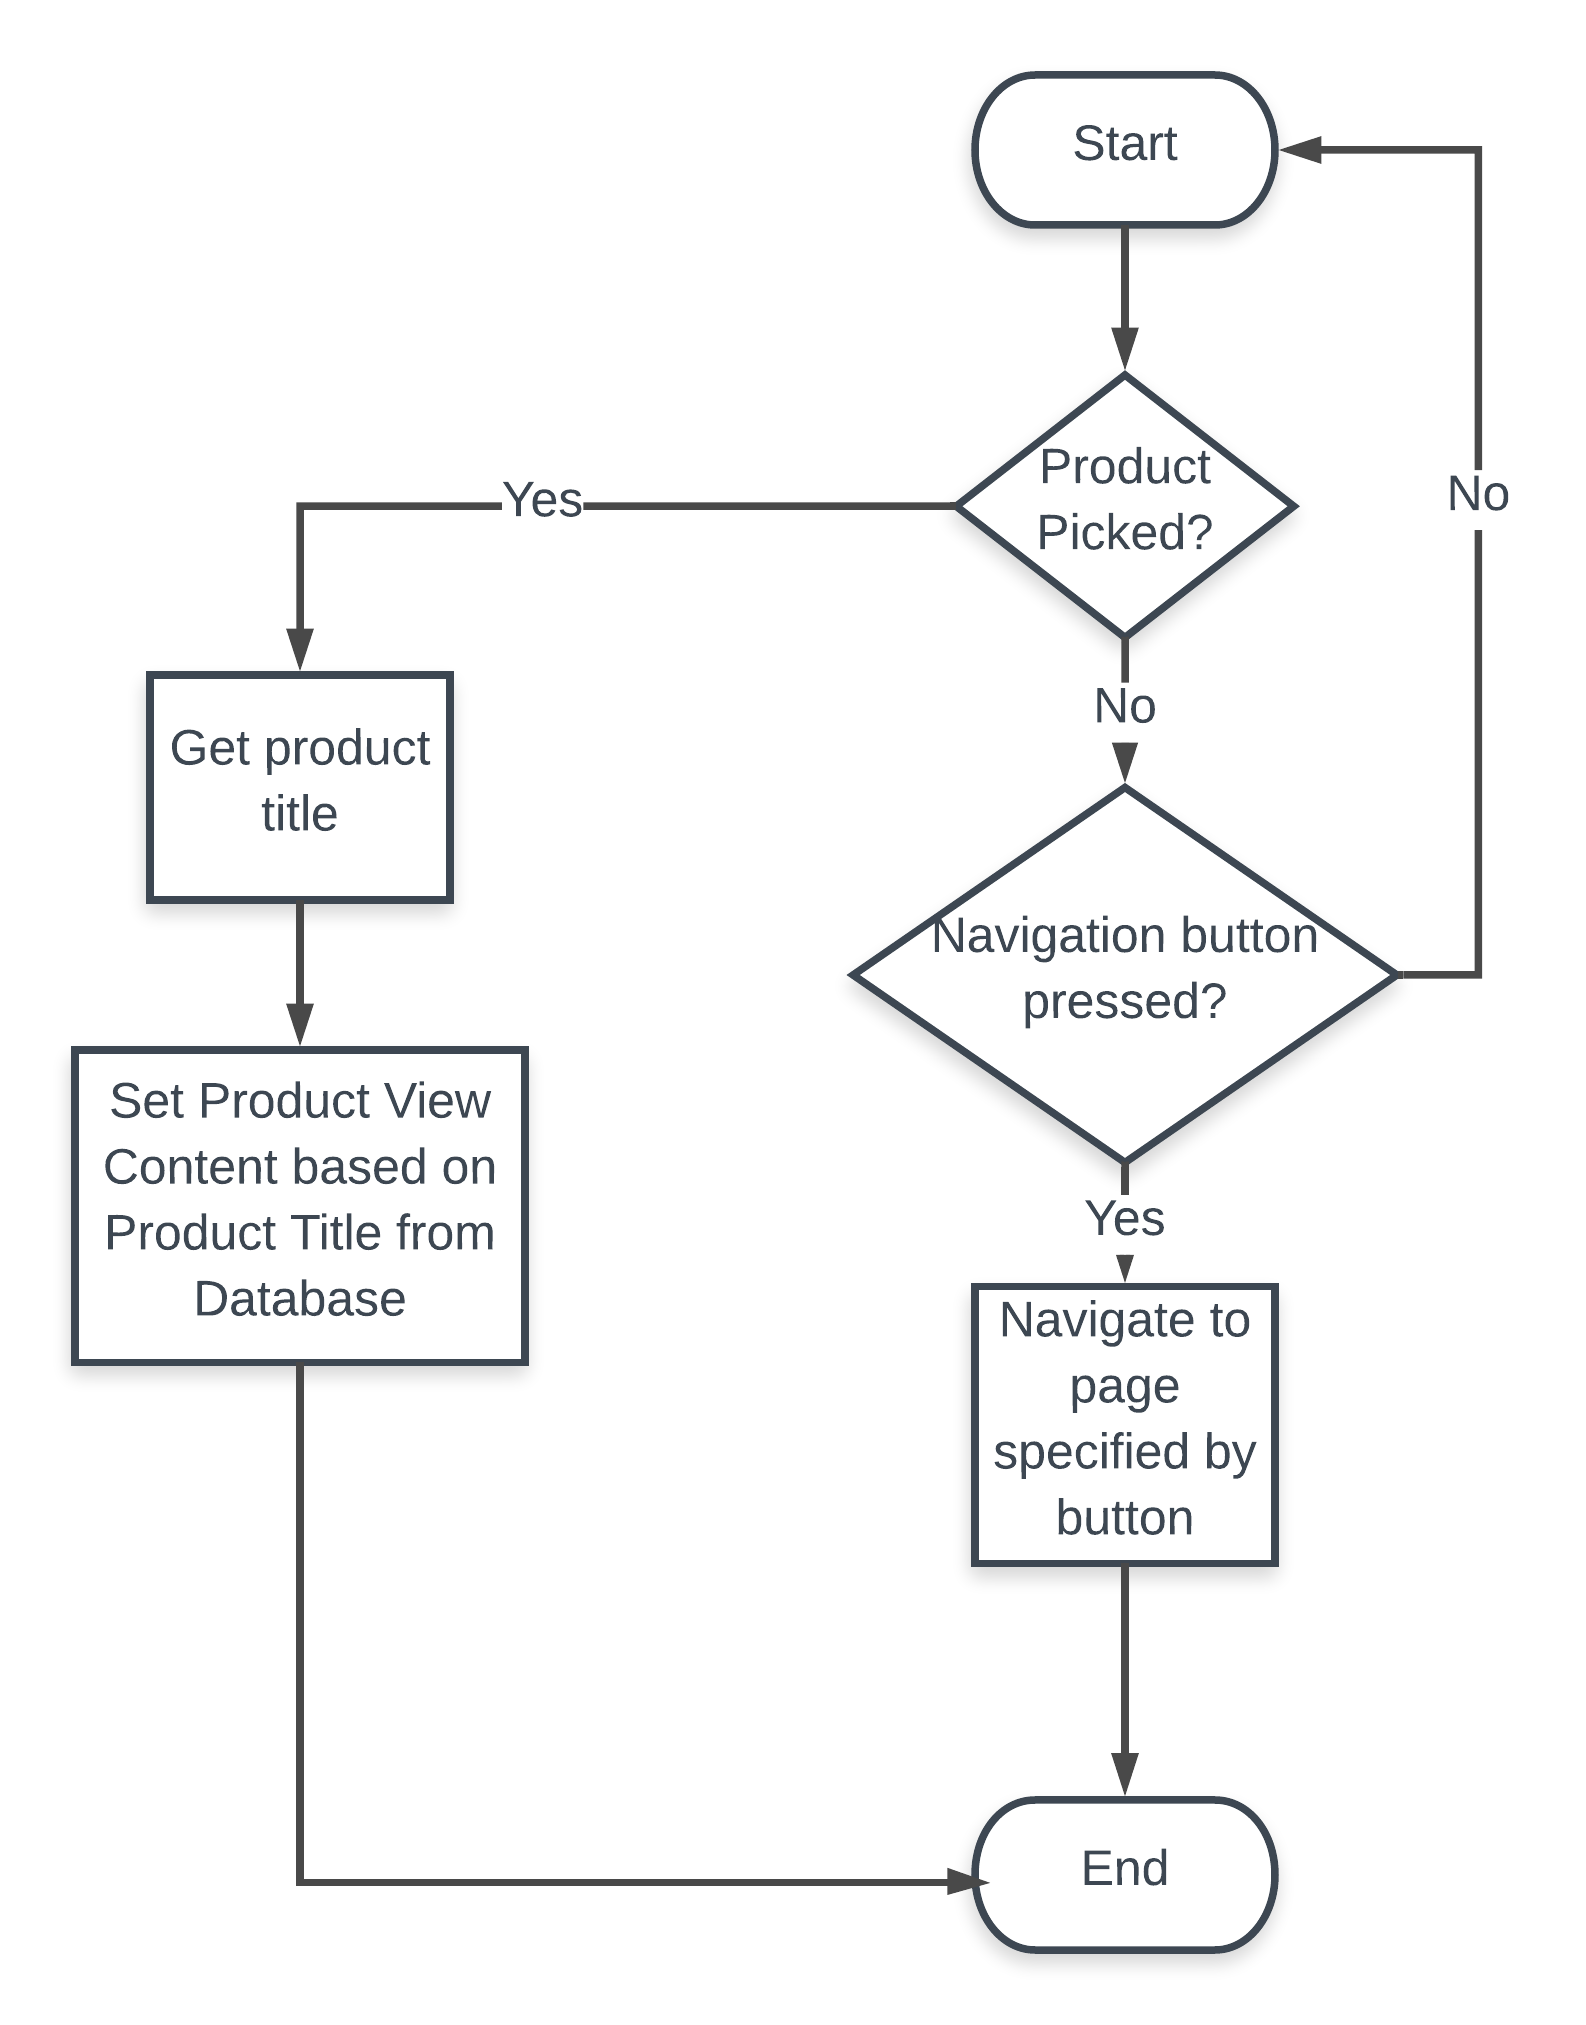
\includegraphics[width=0.9\linewidth]{images/flowMain.png}
\end{center}

\subsection*{Product Information}

\begin{center}
    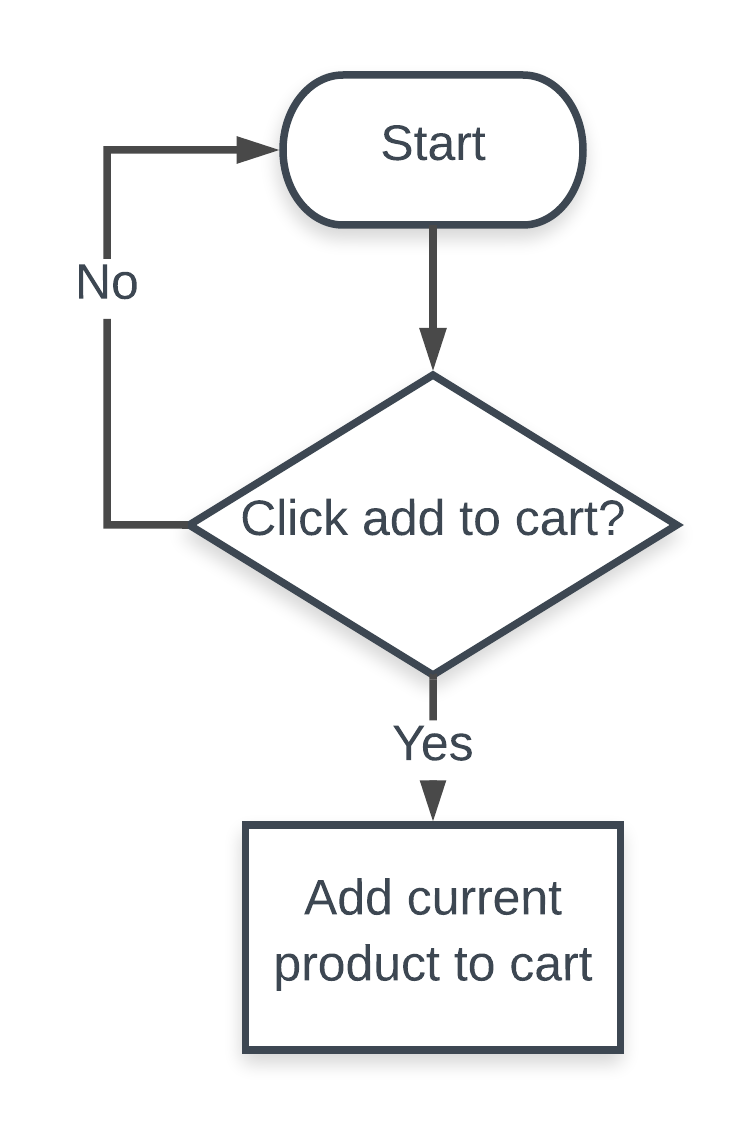
\includegraphics[width=0.5\linewidth]{images/flowProductDetails.png}
\end{center}

\subsection*{Cart}

\begin{center}
    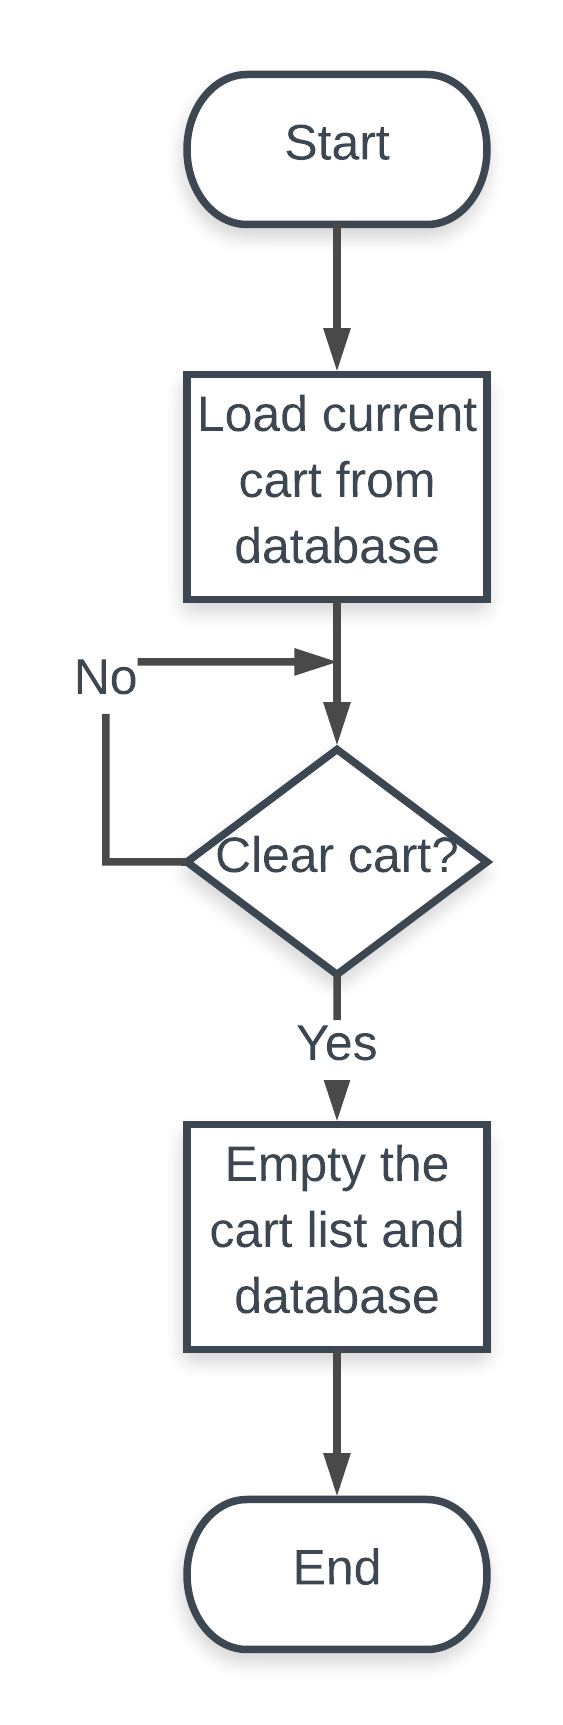
\includegraphics[width=0.4\linewidth]{images/flowCart.png}
\end{center}

\chapter{Development}\label{development}

\section{Introduction}

The development will be carried out in App Inventor which is great software written by MIT in the interest of creating a visual metaphor for programming mobile devices. The programming is carried out through the use of blocks you piece together, using the same conventions as traditional programming languages but without the typing.

\section{GUI Implementation}

App inventor was created with the intention of making app development accessible to all. There are some compromises required to meet that goal, with some of those manifesting in the lacklustre layout management with the software. There is no constraint layout in app inventor, and a lot of view elements that are in android studio simply aren't present in app inventor, restricting what can be achieved with the software with regards to the GUI.

\section{Back-end}

\subsection{Welcome Screen}

When you start the application, you are greeted with this welcome screen.

\begin{center}
    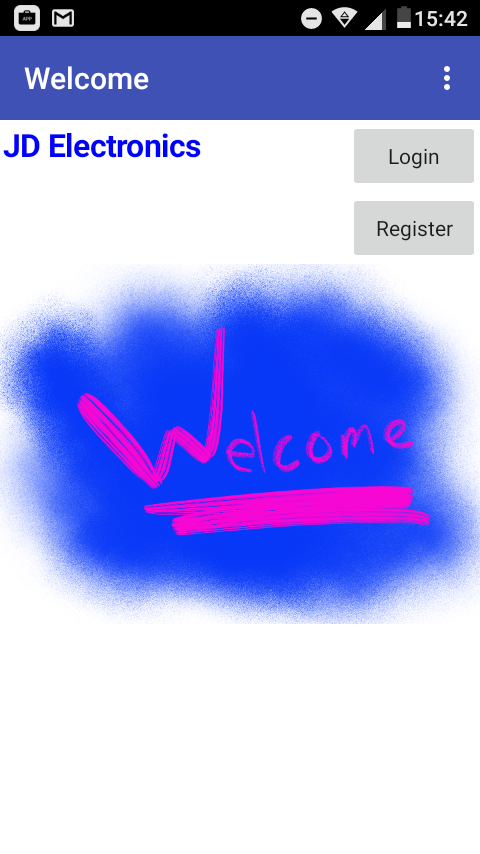
\includegraphics[width=0.5\linewidth]{images/welcomeDesign.png}
\end{center}

This screen presents the user with a welcome message, and a login and register button which leads to a different page. The back-end code for this page is pretty simple, but it's worth showing as it demonstrates a simple event listener.

\begin{center}
    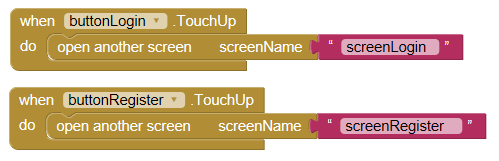
\includegraphics[width=0.75\linewidth]{images/welcomeCode.png}
\end{center}

These events trigger when their corresponding button is touched, and the corresponding screen is then opened. These are the only functions on this page.

\subsection{Register screen}

Clicking the register button on the welcome screen leads here. Here is the design of this screen.

\begin{center}
    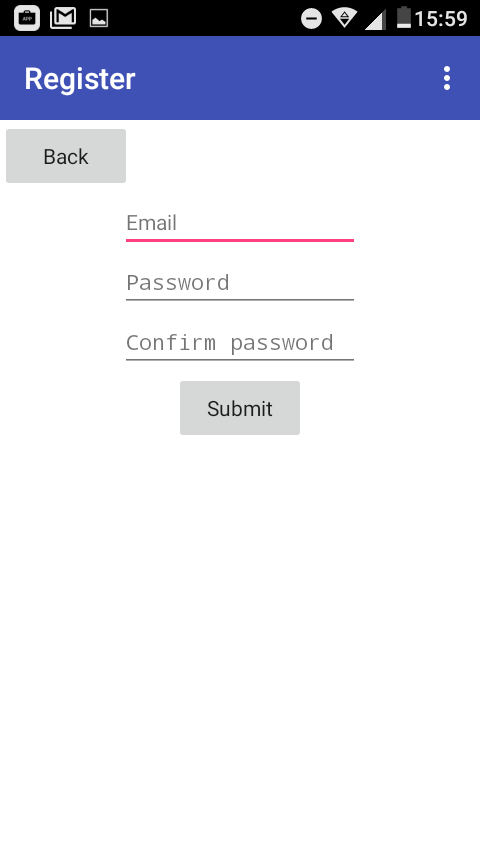
\includegraphics[width=0.5\linewidth]{images/registerDesign.png}
\end{center}

The user inputs their username, and must enter a password twice to ensure that they entered it correctly the first time.

The code is as follows.

\begin{center}
    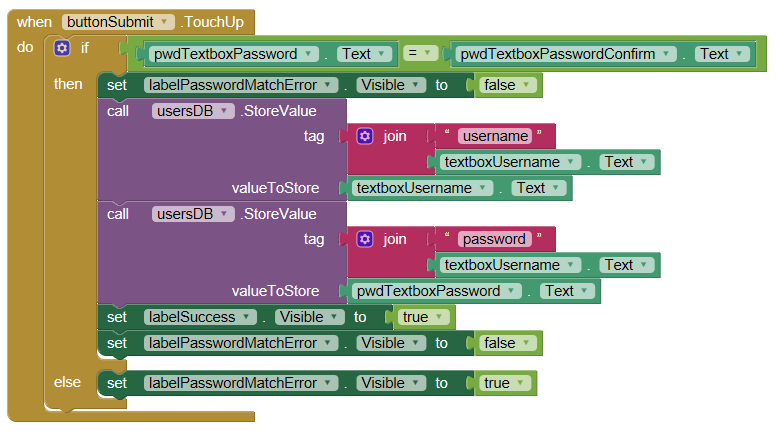
\includegraphics[width=\linewidth]{images/registerButtonSubmit.png}
\end{center}

When the user presses the submit button, the program checks to ensure that the input passwords match and then stores the username and password into a database if the passwords match. The success label is displayed, and if the failure label was visible, it is set invisible. If the password comparison fails, an error label is set to visible.

Other code on this page include the following.

\begin{center}
    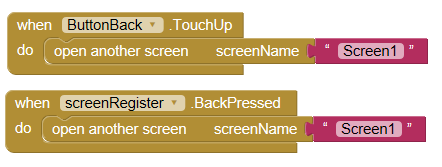
\includegraphics[width=0.75\linewidth]{images/registerOther.png}
\end{center}

This is just simple navigation code to get to the last screen. The only thing of note here is the event listener for the system back button is supported, which leads to the previous page.

\subsection{Login Screen}

The login screen is very simple, with only two text boxes as input, and a login button that executes the logic that checks if the login is valid against the database. The login screen design is as follows.

\begin{center}
    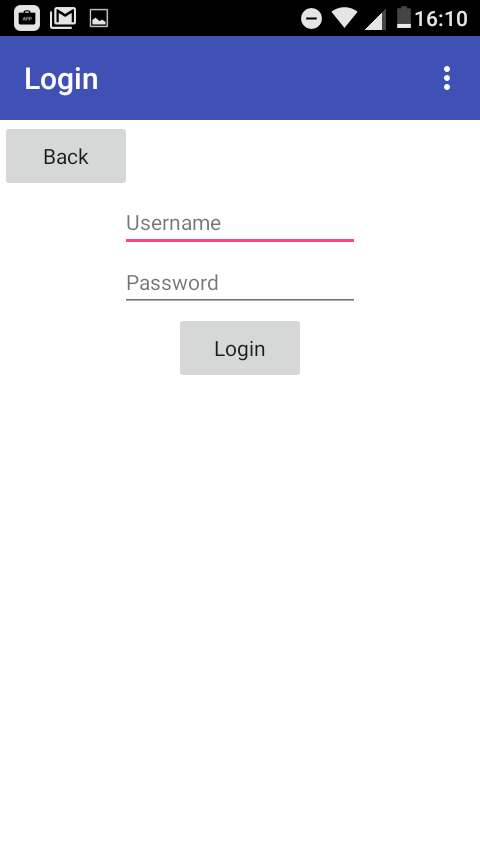
\includegraphics[width=0.5\linewidth]{images/loginDesign.png}
\end{center}

The code for this screen.

\begin{center}
    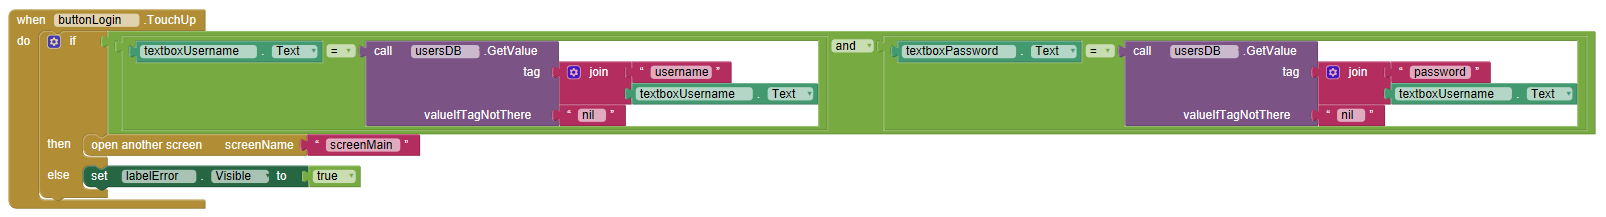
\includegraphics[width=\linewidth]{images/loginButton.png}
\end{center}

This is the code for the login button. This might be too wide to read on the page, but I will describe what it does. When the login button is pressed, the user input username and password is compared against the result of a call from TinyDB on the tag with the `username' or `password' prefix, followed by the user input username. If both comparisons pass, the main screen is opened. If the check fails, an error label is shown.

The following is the rest of the code on the page, boilerplate code.

\begin{center}
    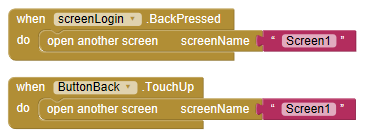
\includegraphics[width=0.75\linewidth]{images/loginOther.png}
\end{center}

\subsection{Main screen}

The primary screen interface consists of a menu bar at the bottom for navigation, a listView in the center containing a list of available products, and a title at the top of the page. I made use of the official google icons for android available at \url{https://material.io/icons/}, which allows you to freely use their high resolution artwork that's suitable for high resolution qHD panels on modern smartphones.

\begin{center}
    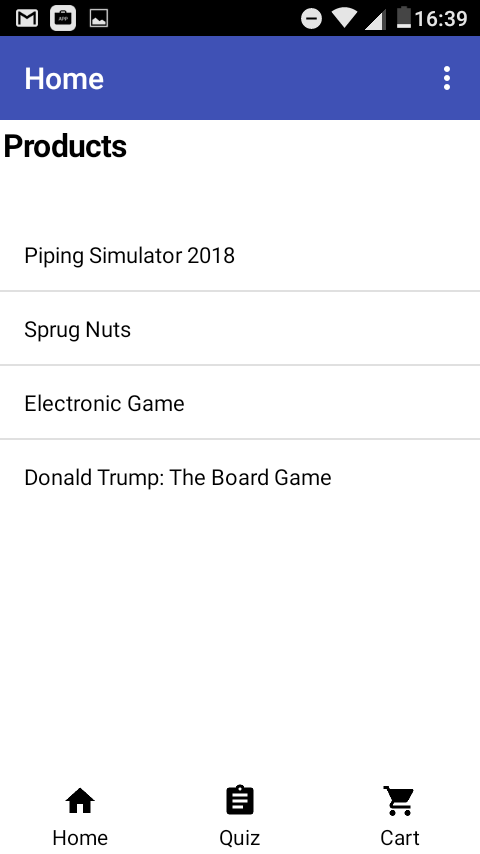
\includegraphics[width=0.5\linewidth]{images/mainDesign.png}
\end{center}

In order to save the product information, I made use of a JSON like data structure so I could easily access the information on a product by parsing a list of key:string pairs. Here is the data structure code block in this screen.

\begin{center}
    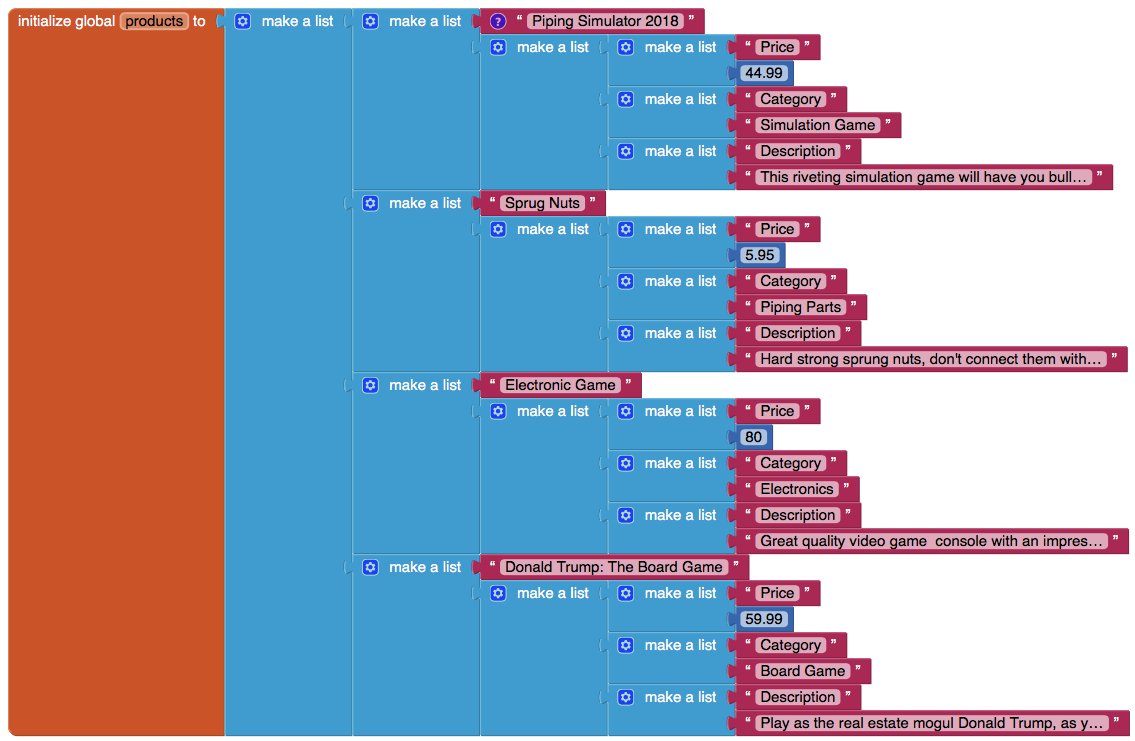
\includegraphics[width=\linewidth]{images/mainList.png}
\end{center}

The whole thing is a list of these key:string pairs. There's a function in app inventor that allows you to search by key to get the string value. List objects in app inventor are actually stored as strings with parenthesis acting as a delimiter between elements of a list, so this works here.

This next part performs the initialization required to display a list of products on the listView in the center of the page.

\begin{center}
    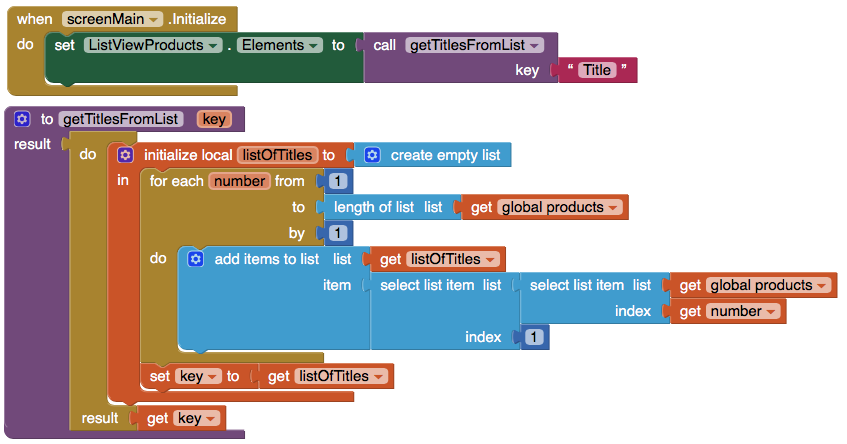
\includegraphics[width=\linewidth]{images/mainInit.png}
\end{center}

The method for extracting just the titles from the great products list is a little verbose, luckily it only needs to be done once, so I put it into its own method for potential reuse later. There is one problem I spotted on review of the code. the \texttt{key} parameter on the function \texttt{getTitlesFromList} isn't used at all in the function.

A run through the code is as follows. I want to create a temporary working list called \texttt{listOfTitles}, instantiating it to an empty list. I then loop through the global \texttt{products} list, selecting the first item on that list (I should replace this select item block with a select with key block to make use of the key parameter of the function), and adding that item to the \texttt{listOfTitles} list. At the end of this, I will end up with a list full of just the titles, and not the other information. At the end of this function, I then return it as output, and in the screen initialize function, this list is passed on as the listViews elements.

These next blocks of code aren't very important, they handle navigation for the bottom navigation bar.

\begin{center}
    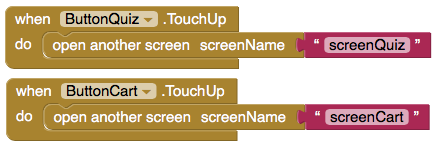
\includegraphics[width=0.75\linewidth]{images/mainNavigation.png}
\end{center}

This last block of code stores the products data and the users selection into TinyDB and opens the product view screen.

\begin{center}
    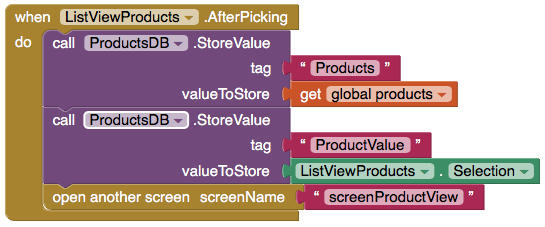
\includegraphics[width=0.75\linewidth]{images/mainDatabase.png}
\end{center}

\subsection{Product View Screen}

\paragraph{Design}

The product view screen required the ability to dynamically change a title, content and price label, as well as an image. The title is at the top, and is in a horizontal layout with the add to cart button to it's right in a vertical layout with a label.

Everything below this is in a vertical scroll layout, with sub layouts in this in order to get a good look and feel.

\begin{center}
    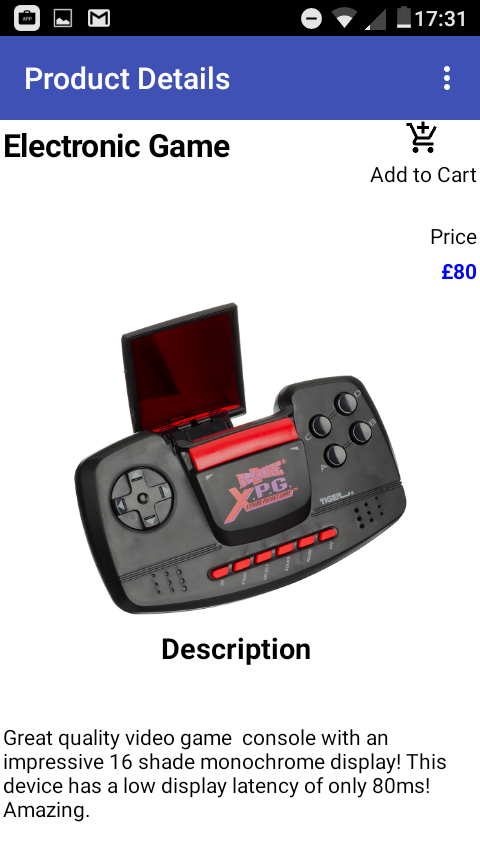
\includegraphics[width=0.5\linewidth]{images/productDesign.png}
\end{center}

\paragraph{Globals}

The first code likely executed on this page is the initialization of the global variables, which are as follows.

\begin{center}
    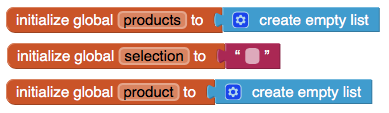
\includegraphics[width=0.75\linewidth]{images/productVariables.png}
\end{center}

TinyDB cannot be a part of the initialization of a variable, so these are initialized to empty lists or strings instead.

\paragraph{Initialization}

The initialization is as follows.

\begin{center}
    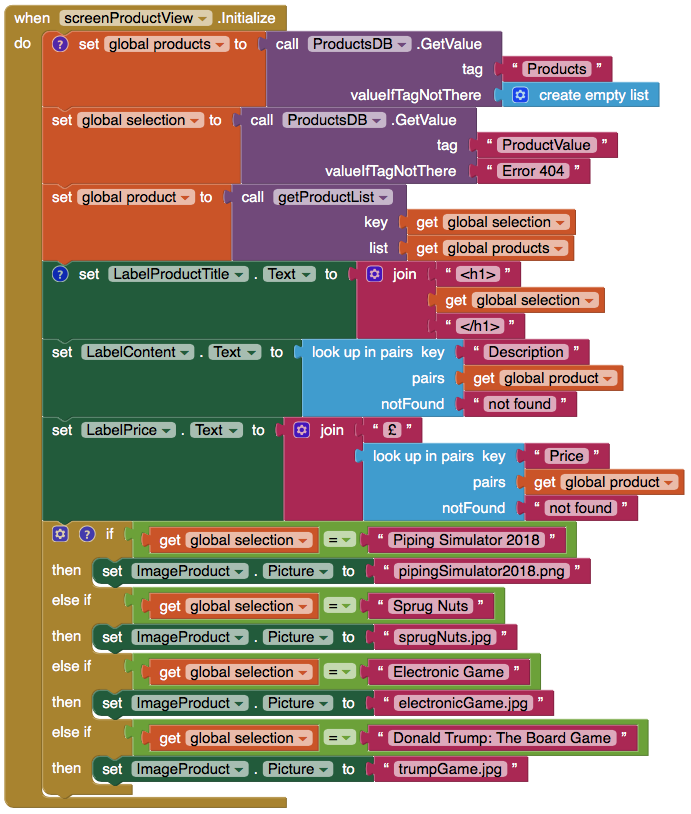
\includegraphics[width=\linewidth]{images/productInit.png}
\end{center}

This is a rather big function call, but once written once it for the most part doesn't need to be touched again. This is with the exception of one thing, that is setting the image. Adding another image to this block isn't complicated, however and only really involves adding two new strings.

At the top I'm assigning the values from the database that were stored in the main page to the globals that were initialized at the start of this page. The top two statements are simple enough, they pull the values from the database at their respective tags, and the third statement gets a sub list using the users selection on the main page as a key to obtain it. This list will contain the product information of the product they had chosen.

The title is easily enough set as it is the same as the global \texttt{selection} variable. The content and price are obtained from the global \texttt{product} list using the appropriate key.

There's a better way to implement the image switching, but the approach that I went for is a large block of conditional statements that checks the global \texttt{selection} string and sets the appropriate image for the picture view.

\paragraph{\texttt{getProductList}}

This next section of the code is responsible for getting a subset for a specific product from the products list.

\begin{center}
    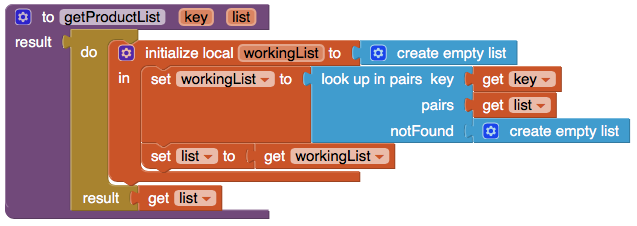
\includegraphics[width=0.9\linewidth]{images/productGetProductList.png}
\end{center}

This function takes the parameters \texttt{key} and \texttt{list}, with the key being the title of the product in that list, and returns a list that contains only key:string pairs for one product.

It does this by using a working list, and creating the subset list using the `look up in pairs' block, and assigning the result to the variable \texttt{workingList}. This list is then returned to the caller.

\paragraph{Add to cart}

The add to cart button action is responsible for adding the currently viewed product to the TinyDB database, and the code for this is as follows.

\begin{center}
    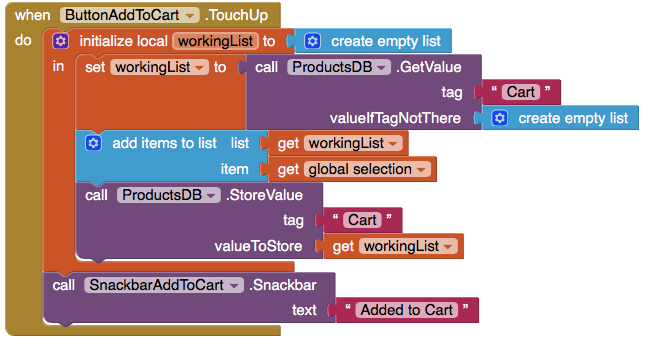
\includegraphics[width=0.9\linewidth]{images/productCart.png}
\end{center}

The code creates an empty working list, and gets the list stored at the \texttt{"Cart"} tag in the TinyDB. The code then adds the current selection to the list, then stores it in the database again with the same tag, overwriting the old list. Outside the scope of the \texttt{workingList} variable, I used an extension to display a small notification at the bottom of the screen to give visual feedback that adding to the cart was successful. A screenshot showing what that looks like is below.

\begin{center}
    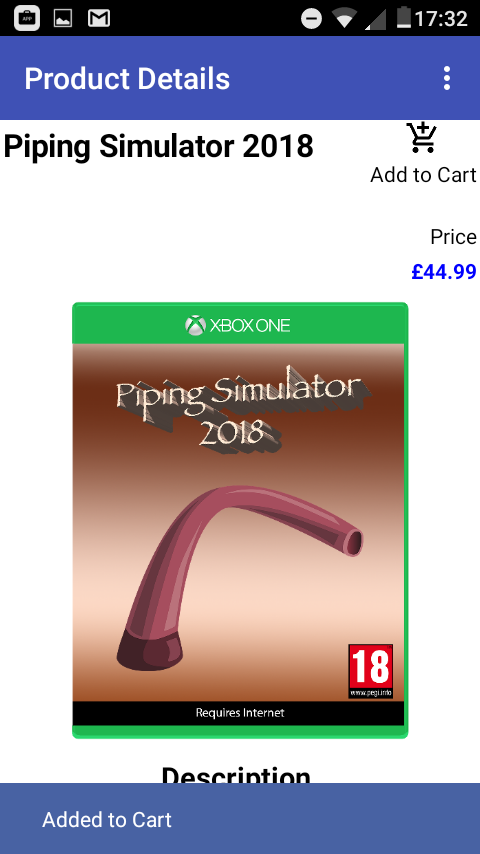
\includegraphics[width=0.5\linewidth]{images/productSnackbar.png}
\end{center}

This notification fades in, has a lifetime or around 1 second, then fades back out without occluding information for too long.

The final bit of code is for navigation.

\begin{center}
    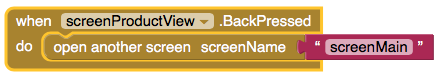
\includegraphics[width=0.75\linewidth]{images/productNav.png}
\end{center}

\subsection{Cart}

The design of the cart is simple because you cannot put images inside listViews like you can with Android Studio. Each cart item in the list view contains a title and a price, and there is also a title label for the page, and a button that clears the cart. The following is what the design of the cart looks like.

\begin{center}
    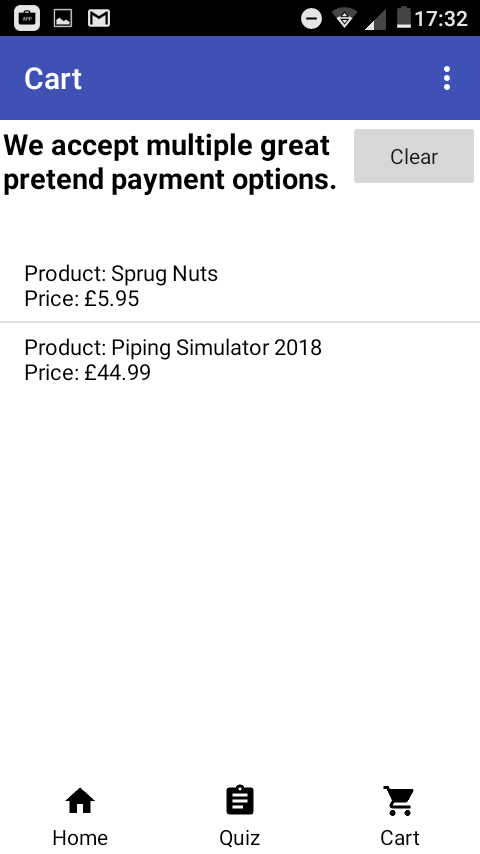
\includegraphics[width=0.5\linewidth]{images/cartDesign.png}
\end{center}

Here's the code for the cart, with the first snippet being the global variables.

\begin{center}
    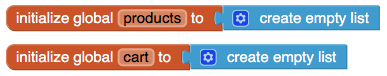
\includegraphics[width=0.75\linewidth]{images/cartGlobal.png}
\end{center}

Much like the page before, we have to initialize these to empty lists because of TinyDB.

\begin{center}
    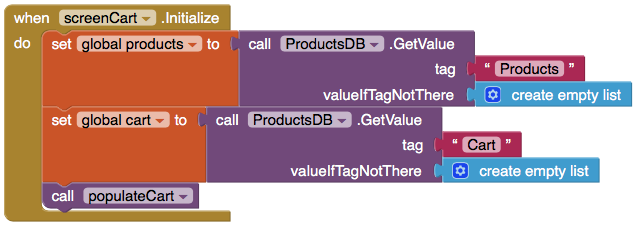
\includegraphics[width=0.9\linewidth]{images/cartInit.png}
\end{center}

This code pull the values from the database into the globals \texttt{products} and \texttt{cart}. This code then calls a function that populates the cart.

This is the code for the function \texttt{populateCart}.

\begin{center}
    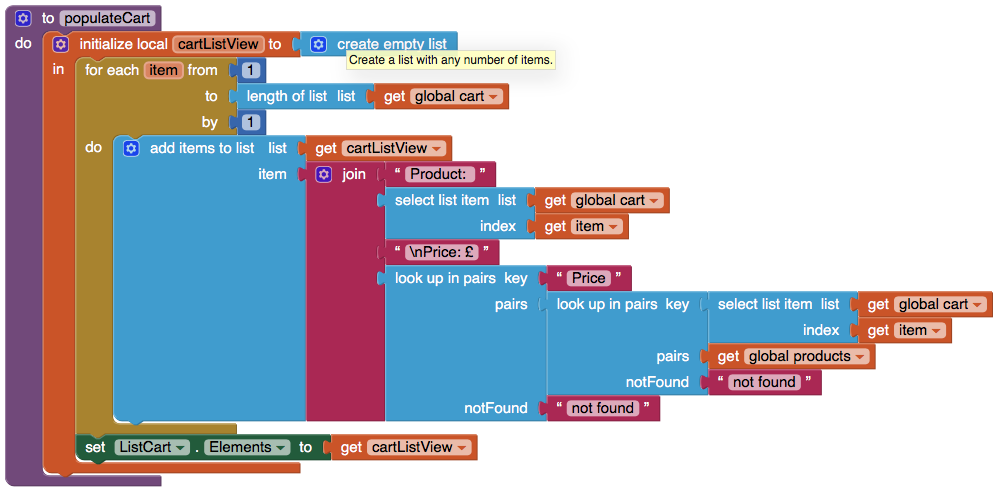
\includegraphics[width=\linewidth]{images/cartPopulate.png}
\end{center}

This function would be the equivalent of void in Java as it does not return a value, but does perform a procedure. The purpose of this function is to get the cart list, and iterate through the product list, on each iteration using the current cart item as an index in the products list and putting these in a string concatenation with an \texttt{\textbackslash n}. These concatenated strings are then passed to a list, and then this list is assigned to a list view to create a cart item entry.

The first three blocks here are responsible for navigation, and the last is responsible for clearing the cart.

\begin{center}
    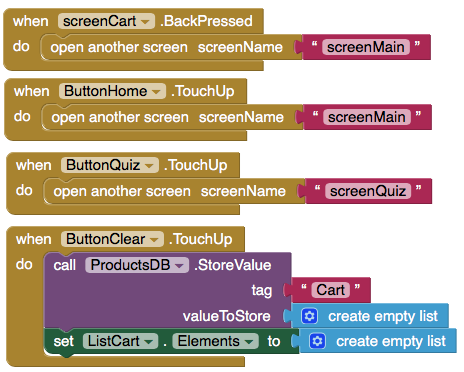
\includegraphics[width=0.75\linewidth]{images/cartNavigation.png}
\end{center}

The clear button just sets the \texttt{"Cart"} tag value to an empty list, clearing it. It also sets the listView elements on the page to an empty list.

\chapter{Testing and Feedback}\label{testing}

\section{Testing}

I was testing for the following in the video below:

\begin{itemize}
    \item All screens start up and function correctly
    \item The registration screen correctly adds a user to the database
    \item The registration screen does not create a user if the passwords do not match
    \item The login screen will not accept a user that isn't in the database
    \item The login screen will accept a user that's in the database
    \item The list on the main screen will populate properly
    \item When the user clicks an item on the list, it should take them to the corresponding product information page
    \item When the user clicks on an item in the bottom navigation bar, it should take them to the corresponding screen.
    \item The product information page should fetch the correct product information from the database and display it correctly
    \item The add to cart button should display a snackbar at the bottom of the screen confirming the add to cart action
    \item Upon the add to cart action, there should be an entry into the cart when the cart screen is loaded
    \item When the clear button is clicked, the cart should be persistently cleared from the list view, and from the database.
\end{itemize}

All of these features appear to work correctly, however when the app is run in the emulator in the video, the list view text and the welcome screen layout display incorrectly. This does not happen when the application is run from a real android testing device, you can look at screenshots earlier in the document under Development to see how they should appear.

The quiz menu item doesn't work as the screen doesn't exist, so should be removed. This was not shown in the video.

\paragraph{Video link}

\url{https://youtu.be/CYf-Gu0mqpk}

\section{Feedback}

\paragraph{Look and Feel}

The feedback I received under this point seems to be generally favorable. The style of the user interface is said to be clean and consistent, however I have received on criticism with regards to the plain presentation of the main menu screen. There is no thumbnail icon for each of the products. In order to maintain compatibility with the code I would have to ensure that I am still using a list view, however there is likely third party app inventor extensions that would allow me to present images alongside the text elements.

\paragraph{Functionality}

The login and logout function was received to be potentially useful in a full app, and the add to cart snackbar was seen to be a nice addition to the application, with the snackbar said to be useful elsewhere, especially if pared with a button such as undo.

\paragraph{Purpose}

The reason for the apps existence was perceived to be clear, with the application being a commerce app, There weren't many issues there. It was said however that the app could do with some extra functionality, with features such as search, filtering and categorization of products being a potential addition in the future.

\chapter{Deployment Presentation}\label{deployment}

Refer to the attached slides.

\printbibliography

\end{document}
